\chapter{Literature Review} % Main chapter title

\label{Chapter2} % For referencing this chapter elsewhere, use \ref{Chapter2}

\lhead{Chapter 2. \emph{Literature Review}}

%----------------------------------------------------------------------------------------
%	SECTION 1
%----------------------------------------------------------------------------------------

\section{Background}

The question of the representation of numbers as we, humans, use them in a world of electronics has been central in the creation of computers and their associated arithmetics. Several problems are contained in the simple question of: How to translate our arithmetic and number operations in a piece of hardware?

%-----------------------------------
%	SUBSECTION 1 - Number Representation
%-----------------------------------
\subsection{Number Representation}

The first thing to note is that electronics can represent two states, a presence or absence of an electric impulsion. The states of \guille{on} and \guille{off} is embedded in transistors that can represent both. The transistor is the hardware representant of this duality while a bit is the software counter-part. This is the underlying reason of why computers, even the first fully electronical computer ENIAC (\emph{Electronical Numerical Integrator and Computer}), are using a binary system. If this system is handy to translate our base 10 arithmetic and simple numbers such as integers, it is harder to translate more complex numbers such as reals and floating point operations. The meaning of an N-bit binary word is entirely dependent of the interpretation we choose to use. This interpretation consists of both a representation (the type of the object the memory represents) as well as its associated mapping. Common number representations consists of unsigned integers, signed integers (using two's complement), floating point reals as well as fixed-point reals.

%-----------------------------------
%	SUBSUBSECTION 1 - Integer Representation
%-----------------------------------
\subsubsection{Integer Representation}

The representation of integers and especially unsigned integers is straightforward as it consists of a change form base 10 to base 2. This number representation can be done in 16-bits, 32-bits or 64-bits depending on its type, the supporting hardware and the space we need to contain it. Representing a number in base 2 from base 10 or vice versa is straightforward as it only demands simple and exact basic operations to be performed.

% EXAMPLE INTEGER REPRESENTATION
% \begin{figure}[htbp]
% 	\centering
% 		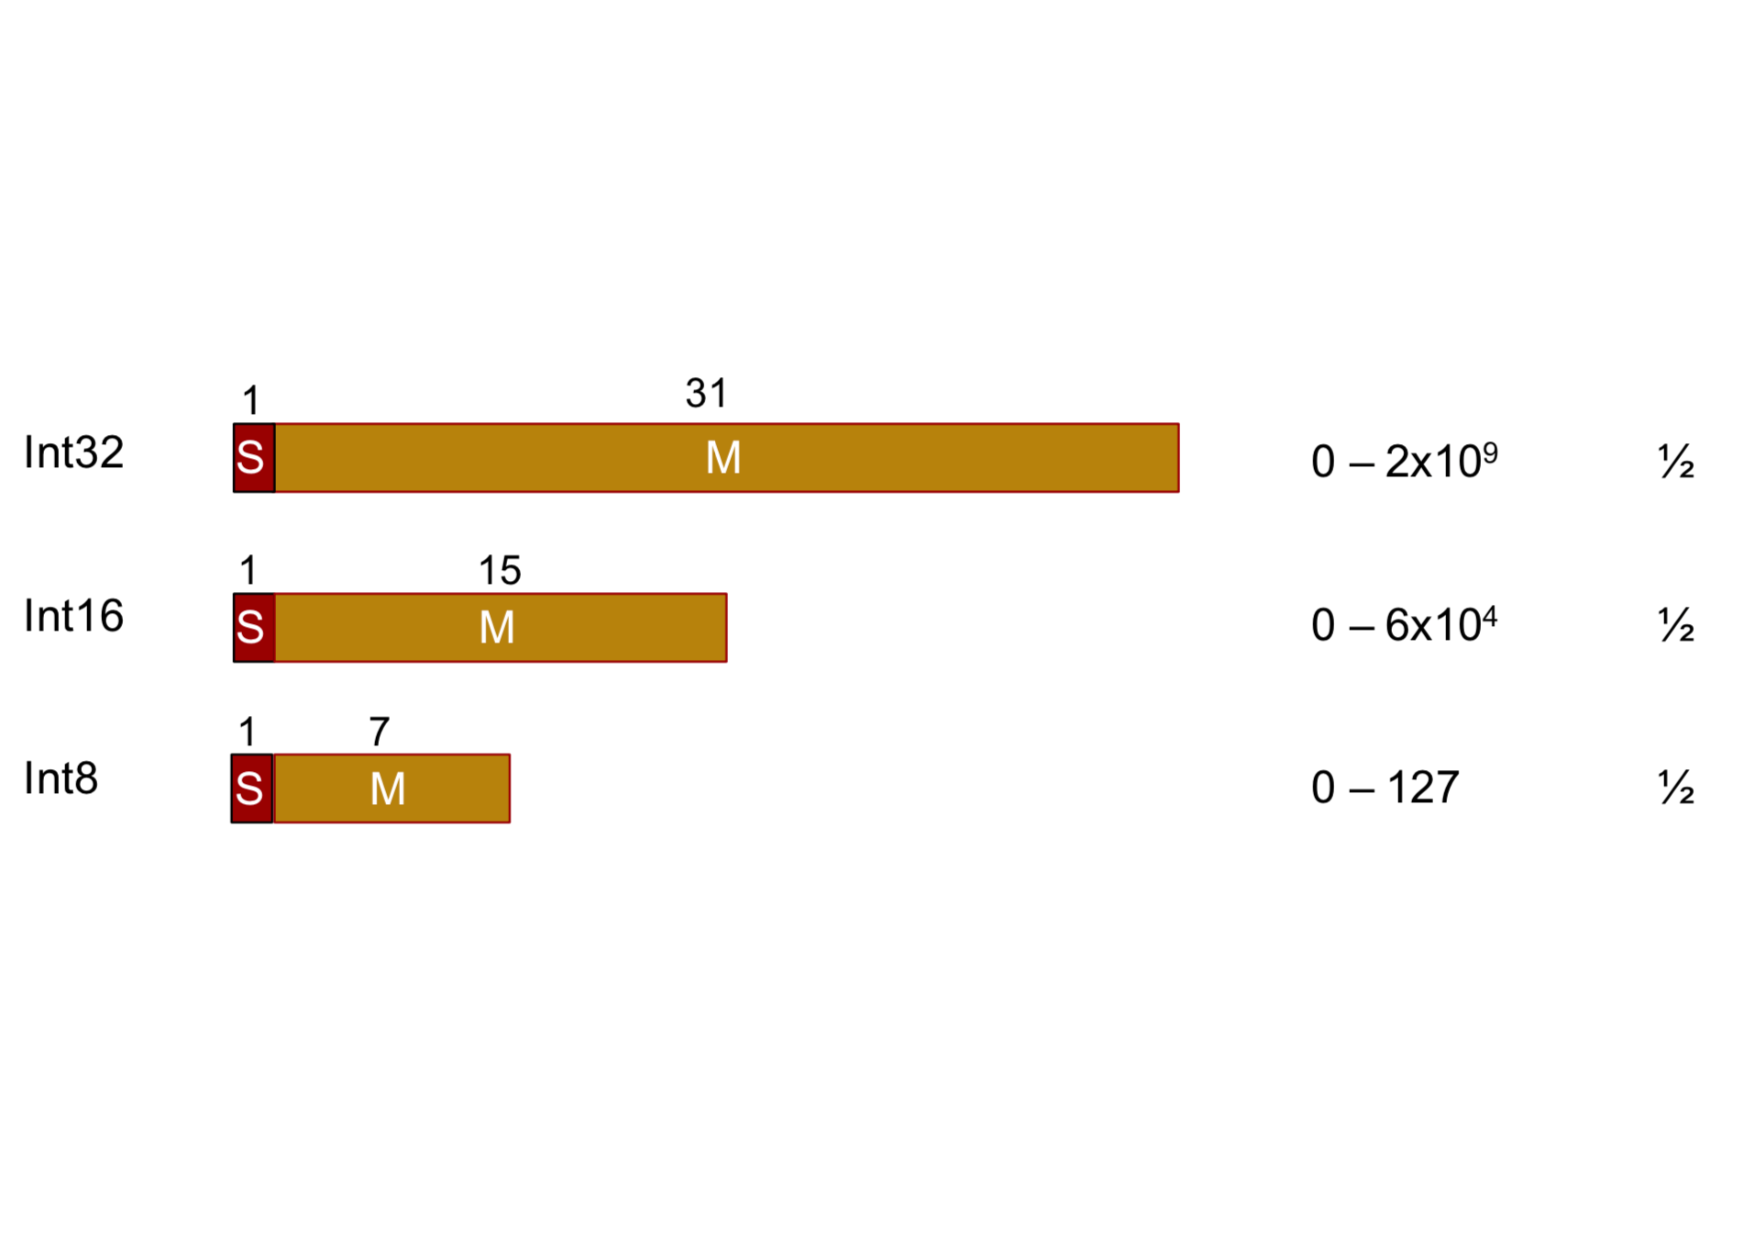
\includegraphics{Figures/IntegerRepr.pdf}
% 		\rule{35em}{0.5pt}
% 	\caption[Integer Representation]{Example of the representation of an integer}
% 	\label{fig:IntegerRepr}
% \end{figure}

Now, if we want to represent a signed integer, we have to use a method called the two's complement in order to bring the sign in while keeping the basic behavior of the addition to work on numbers whether they are positive or negative. The method consists in changing the value of all the bits of a given number then adding one to the result.

% EXAMPLE TWO'S COMPLEMENT
% \begin{figure}[htbp]
% 	\centering
% 		\includegraphics{Figures/TwosComplement.pdf}
% 		\rule{35em}{0.5pt}
% 	\caption[Two's Complement]{Example of the two's complement}
% 	\label{fig:TwosComplement}
% \end{figure}

Those two representations allow a complete mapping of integers up to a certain range: signed 32-bit integers can represent base 10 numbers between -2,147,483,648 and 2,147,483,647 while unsigned integers can represent base 10 numbers between 0 and 4,294,967,295.

%-----------------------------------
%	SUBSUBSECTION 2 - Floating-Point Representation
%-----------------------------------
\subsubsection{Floating-Point Representation}

Representing floating-point numbers has been a concern since the 1980's and the industrial development of several computing modules and interfaces. The need for a consensus in this domain and particular applications has been answered by the IEEE-754 standard \cite{Ieee754} in 1985. This standard defines both the floating-point number representations and exceptions conditions along with their default handling. This norm was reviewed fondamentally in 2008, extending it to 64-bits and 128-bits length. The last dated revision of the norm is from 2019.

Floating-point numbers following this representation are composed of three distinct elements:
\begin{enumerate}
  \item A sign bit
  \item An exponent
  \item A mantissa
\end{enumerate}

Those three elements compose the number by using the following formula:
\begin{equation}
  (sign)\ mantissa \times 2^{exponent}
\end{equation}

In order to present both positive and negative exponents and as using the two's complement on the exponent would complexify the computation of floating-point numbers, a bias is used in the exponent. This bias corresponds to:
\begin{equation}
  2^e - 1
\end{equation}
where e is the number of bits of the exponent part.

When referring to single-precision floating-point representation we are talking about 32-bit long memory representation. They are mapped as follows:
\begin{itemize}
  \item Sign bit: 1 bit
  \item Exponent: 8 bits
  \item Mantissa: 23 bits
  \item Exponent Bias: 127
\end{itemize}

% FP32 EXAMPLE
% \begin{figure}[htbp]
% 	\centering
% 		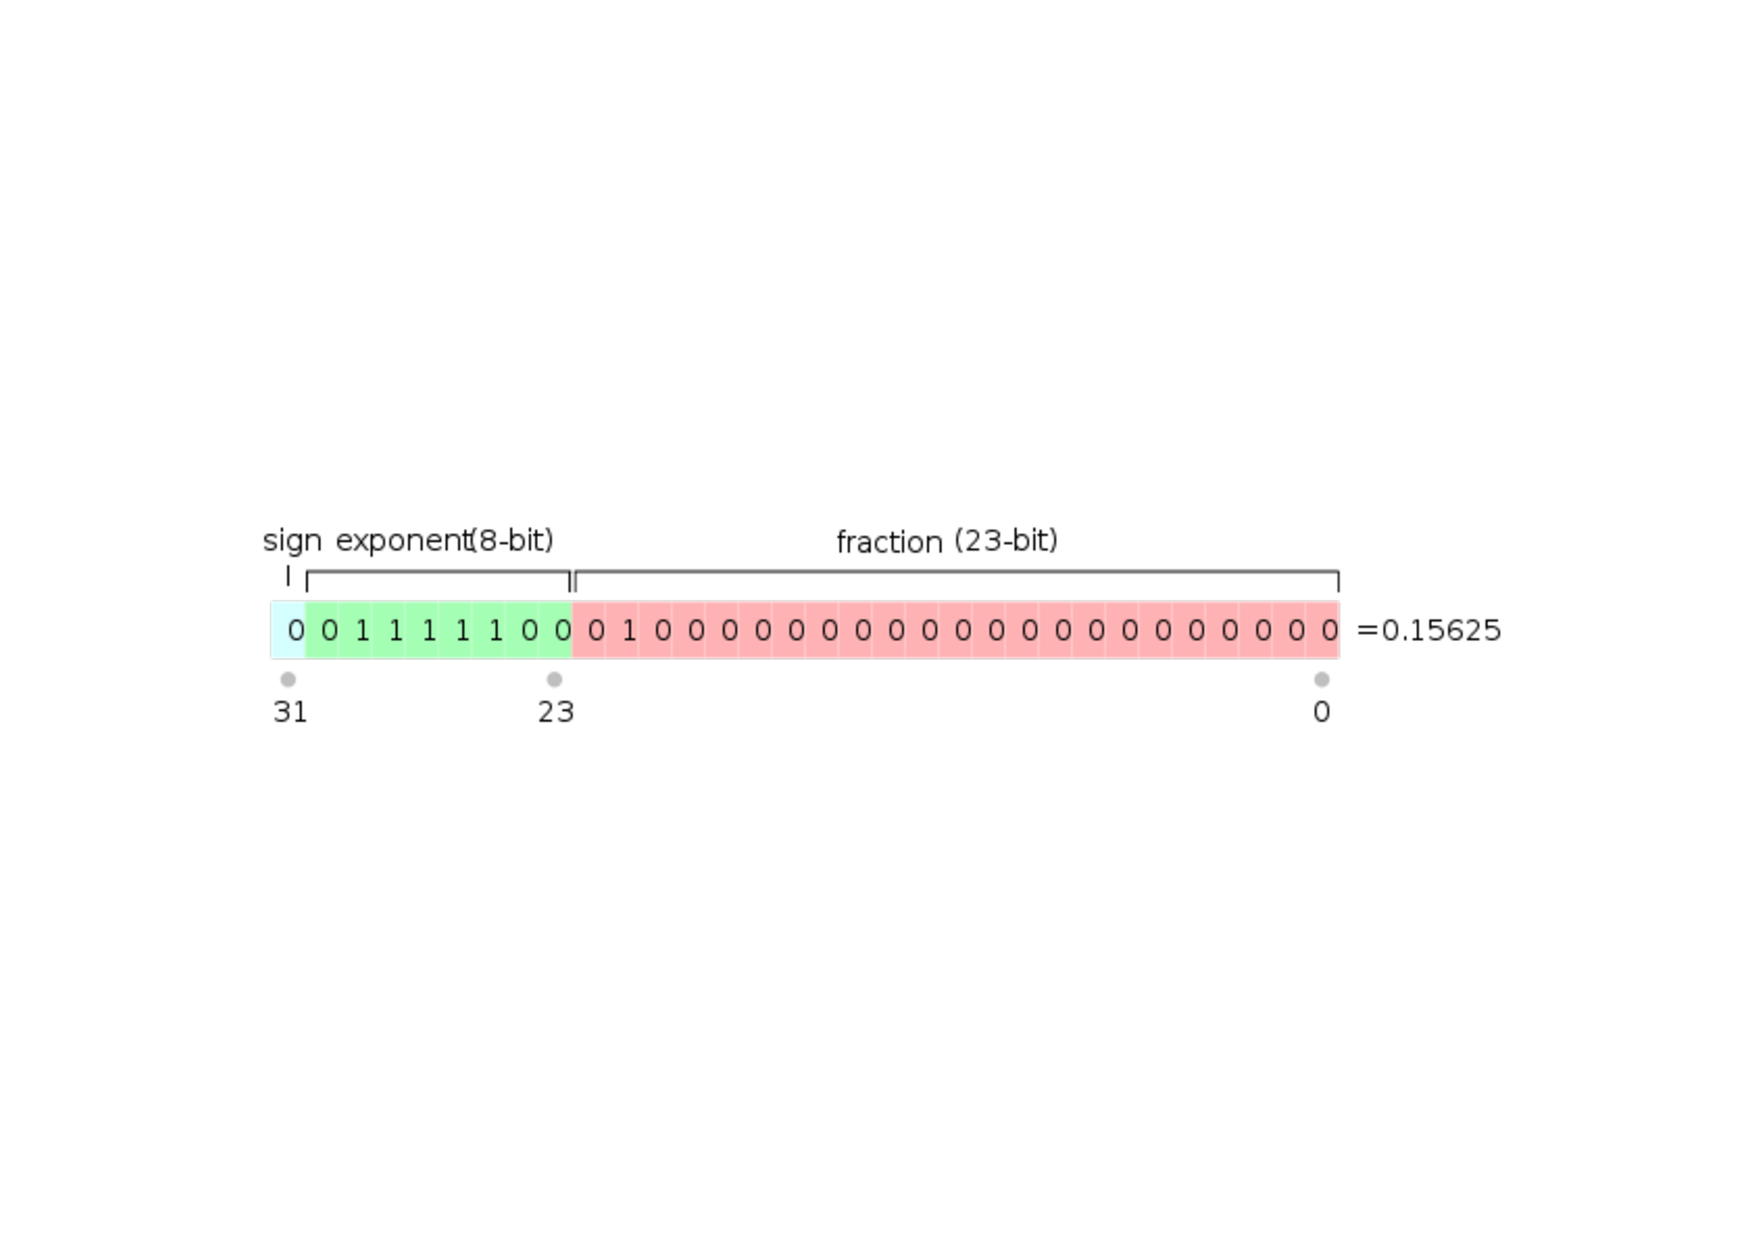
\includegraphics{Figures/SPFP.pdf}
% 		\rule{35em}{0.5pt}
% 	\caption[Single-precision float representation]{Example of the representation of a float in single-precision}
% 	\label{fig:IntegerRepr}
% \end{figure}

Referring to double precision floating-point representation means looking at 64-bit long memory representation, mapped as follows:
\begin{itemize}
  \item Sign bit: 1 bit
  \item Exponent: 11 bits
  \item Mantissa: 52 bits
  \item Exponent Bias: 127
\end{itemize}

% FP64 EXAMPLE
% \begin{figure}[htbp]
% 	\centering
% 		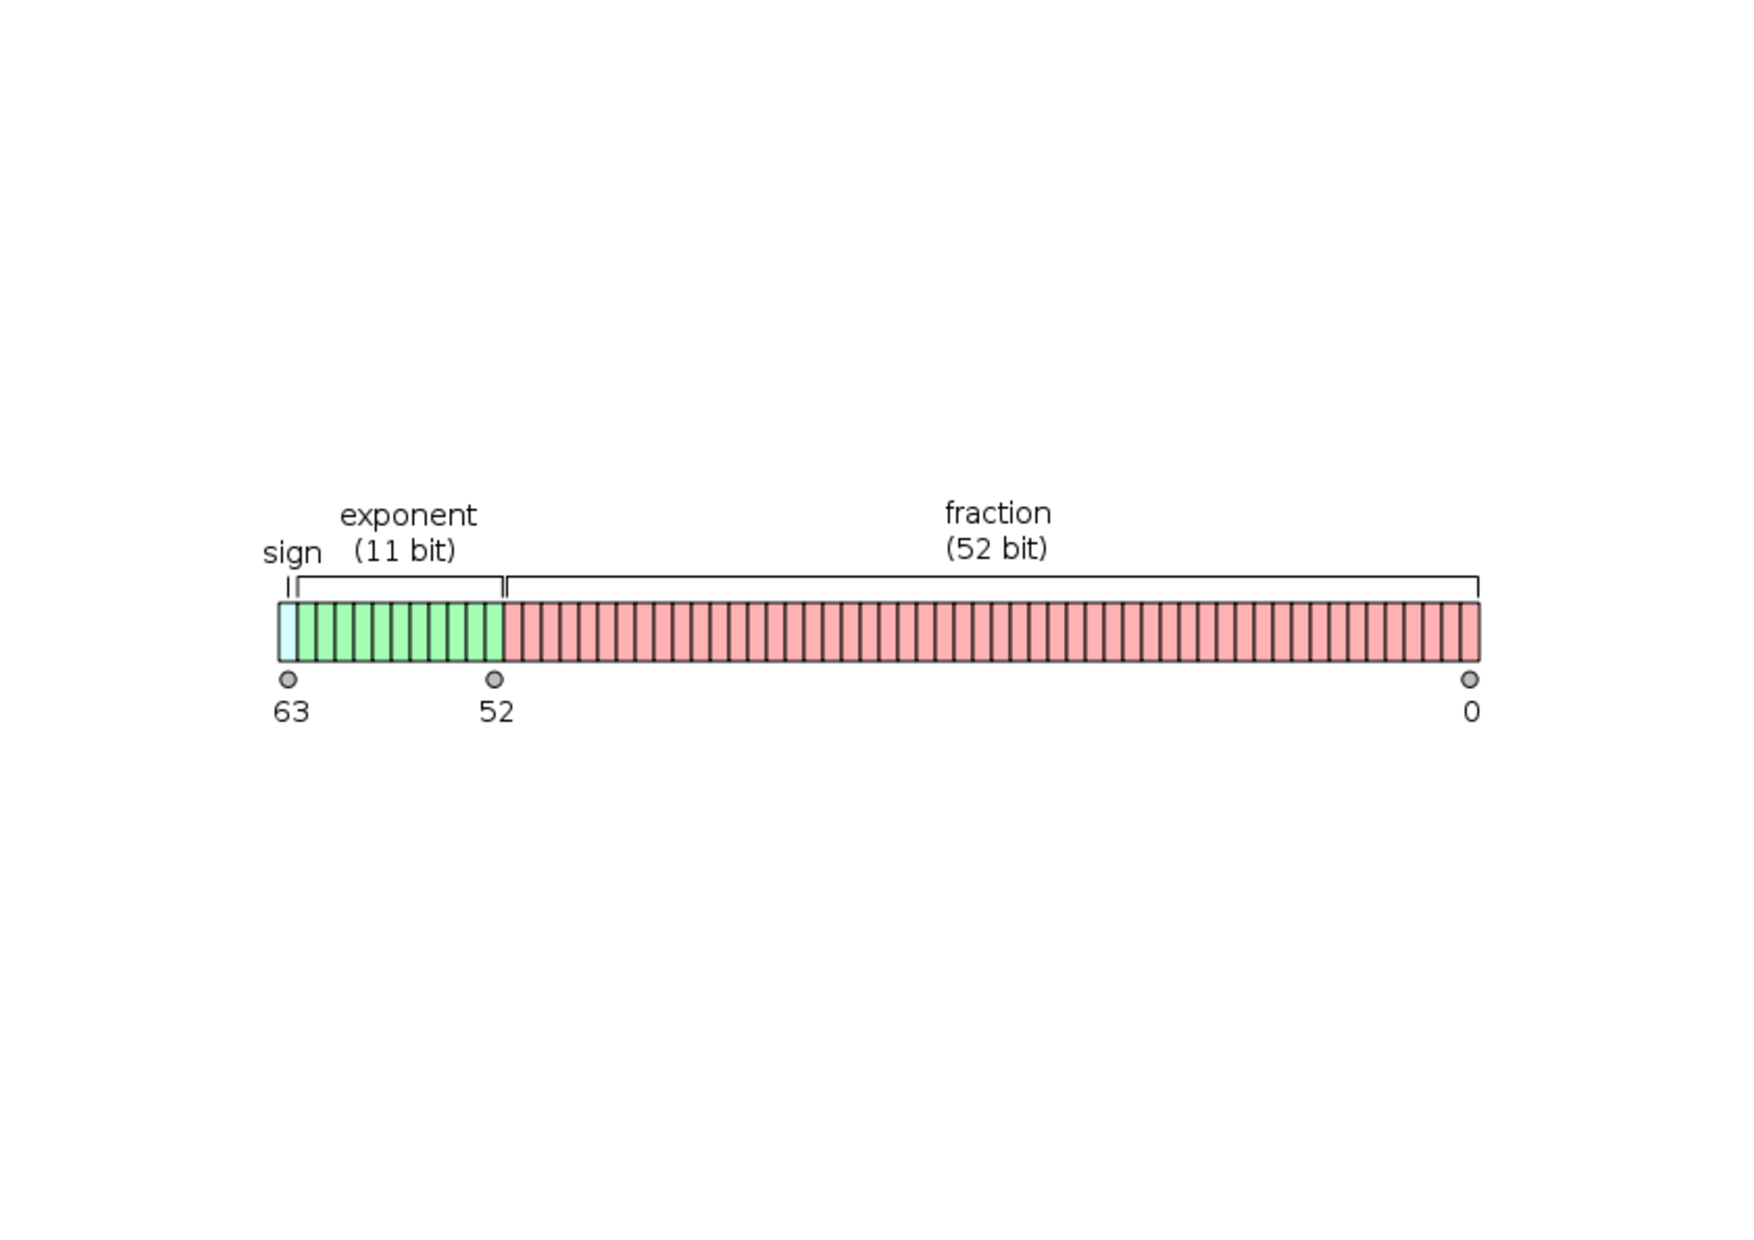
\includegraphics{Figures/DPFP.pdf}
% 		\rule{35em}{0.5pt}
% 	\caption[Double-precision float representation]{Example of the representation of a float in double-precision}
% 	\label{fig:DPFP}
% \end{figure}

Along this representations, IEEE-754 introduces representations of special numbers such as positive and negative infinity as well as NaN and zero. Moreover, it adds methods to round floating-point numbers to positive or negative infinity, zero or to the nearest value.

%-----------------------------------
%	SUBSUBSECTION 3 - Fixed-Point Representation
%-----------------------------------
\subsubsection{Fixed-Point Representation}

Another way to look at the decimals is to fix the radix point to be at a certain place and keep it thoughout all the computations and representations using this arithmetic. A fixed-point representation consists of three components:
\begin{enumerate}
  \item A sign indicator
  \item An integer corresponding to the total number of bits
  \item Another integer corresponding to the size of the fractional part
\end{enumerate}

Representing a number with this representation can be done by simply concatenating the base 2 representation of each side of the radix point.

% FIXED POINT EXAMPLES (SEVERAL EXAMPLE OF THE SAME NUMBER)

As shown in the above example, several representations can depict the same decimal number. Finding the correct amount of bits to allocate to each side of the radix point is what will qualify the representation. Allocating fewer bits than needed may lead to overflow while allocating too much may increase quantisation errors.
Along with this new representation comes a whole new arithmetic. While this format can help tailor your needs in terms of variable types, it comes with an additional cost. The operations performed in this arithmetic are non-trivial as addition and multiplication are not associative and distributive anymore. This means the order of the operations will have an impact on the final result. Moreover, the round-off error underlying this representation is often non-trivial to grasp. However, those operations are low demanding in terms of computing power.

%-----------------------------------
%	SUBSECTION 2 - Performance Benchmarks
%-----------------------------------
\subsection{Performance benchmarks}

Floating-point representation (in either single or double precision) allows extreme precision at the cost of space in memory. On the other hand, fixed-point representation, even if it comes with a more complex arithmetic and insidious round-off errors, allows to tailor the type to your needs. If you want to store the values of the size and mass of planets in floating-point precision, you will end up not using the majority of the range of values you selected while you could tailor a correct type in fixed-point representation.

The operations performed in floating-point are expensive in terms of bandwidth, memory and energy consumption, which ultimately translate in to additional cost to perform an action. Mark Horrowitz talk at the ISSCC 2014 was entitled \guille{Computing's Energy Problem (and what we can do about it)} provides an insight of the problems and challenges technology scaling has encountered in its development. Moore's law is getting outdated and a solution to the issue of permanently growing energy needs resides in \guille{the design of applications and hardware that are better matched to task and each other}. The numbers presented by M.Horrowitz have been reused by Professor William Dally (Standford University, NVidia Corporation) in his lecture on \guille{High-Performance Hardware for Machine Learning} \cite{Nips2015}. The following graph is extracted from this lecture and presents the energy and area costs different floating-point operations demand.

% COSTS OF OPERATIONS 2015-DALLY

The benefit of using a more optimised representation other the floating-point representation has been investigated as soon as in 2000 in 2000-TONG. The authors present a way to reduce the energy consumption by minimising the bitwidth representation of the floating-point data. The data used to tailor the type representation is human-sensory data such as speech or video imagery. This kind of data is obtained at low precision (4 to 10 bits) but mapped into a full single-precision floating-point type. Using such optimisations, the authors manage to obtain a reduction of 66\% in multiplier energy per operation without sacrificing any accuracy.

Xilinx, a manufacturer of Field-Programmable Gate Arrays (FPGAs), produced a white paper written by Finnerty et al. \cite{Xilinx2017}. This paper shows that the tools Xilinx provide can already handle fixed-point types and arithmetic and that the benefits are important for use of the FPGA:
\begin{itemize}
  \item Reduced power consumption
  \item Reduced use of FPGA resources (look-up tables, flip-flops, memory)
  \item Latency improvements
  \item Comparable performance and accuracy
\end{itemize}
The authors show the example of an FIR filter implementation in fixed-point representation from floating-point. The frequency is shown to be 16\% faster and the latency 7.5 times lower.

In conclusion, using a type that matches correctly the use you will make of it in an environment where costs are translated in terms of energy consumption, memory or bandwidth usage, will always come out as an improvement with little to no loss in accuracy.

%----------------------------------------------------------------------------------------
%	SECTION 2
%----------------------------------------------------------------------------------------

\section{Mixed Precision}

The previous section explained in details the different existing number representations. With a particular emphasis on the representation of floating-point number, the previous section has shown what the underlying issues of such representations are. The question now is how can we use to our advantage the different types along with their strengths and weaknesses?

%-----------------------------------
%	SUBSECTION 1 - Motivations
%-----------------------------------
\subsection{Motivations}

The term \guille{mixed precision} comes from the idea of using different precisions (type representations) to increase the performance of a computation that would otherwise only use the highest available (or user-defined) precision. The previous section shown us that each number representation has its pros and cons. Using lower precision types and representations will allow the total computation to decrease the usage of several hardware resources (memory, bandwidth, energy consumption) \cite{Horowitz2014,Nips2015}.

However, if lower-precision is acceptable, using mixed-precision can increase the capacity of smaller systems and subsystems as it will increase the overall performance and resources usage. This goal is targetted when you are aiming for the most performant processor, being given a size and type of usage. Moreover, this can be used when you know exactly the tasks your system will perform as well as their needed size. Yates \cite{Yates2007} presents several rules allowing you to determine the required size of any operation performed in fixed-point arithmetic. This arithmetic, as shown earlier is an interesting choice as it allows you to tailor the type to your needs. Reconfigurable hardware can take advantage of this as well by using the exact required size for an operation. Such architecture will be looked upon on the next sections.

Scientific computations often require the highest available precision and the reduced precision induced by the lower-precision components is unacceptable. In order to still take advantage of the several gains lower-precision provides, a compromise has to be found about how and when to use lower-precision. Ideas on the usage have been looked upon since the 1950's and the first methods to correctly implement them in the early 1960's.

In any case, the developer has to know and keep in mind:
\begin{itemize}
  \item Required end precision
  \item Acceptable error rate
  \item Actual operations performed by the system
\end{itemize}

Mixed precision methods consist of doing a large part of the computation in low-precision components and only a small part in high-precision. As presented in the survey paper \cite{Goddeke2007} using different formats in the same algorithm can have several beneficial properties such as:
\begin{itemize}
  \item Accuracy: Same accuracy when up to 99\% of the operations is performed in the low format
  \item Computation: Low precision operations require less transistors and can translate in more paralellism
  \item Memory: Reduction in size in memory influences the efficiency and bandwidth requirements positively
\end{itemize}

%-----------------------------------
%	SUBSECTION 2 - Methods and Implementations
%-----------------------------------
\subsection{Methods and Implementations}
Several methods to actually implement a mixed precision algorithm have been developed starting 60 years ago. If the methods are different in practice, the theory behind them is the same as they aim to delegate most of the work to low-precision components while only using high-precision to recover the desired accuracy for the computation.
%-----------------------------------
%	SUBSUBSECTION 1 - Iterative Refinement
%-----------------------------------
\subsubsection{Iterative Refinement}

Since the early 1960's, literature has studied the effects and ways to implement mixed precision. The first known works to implement such methods is 1963-Wilkinson and 1967-Moler. The method presented by both is named \guille{iterative refinement} and uses a combination of accumulative inner products along with a linear solver. This solution is directed towards the resolution of a system in the form of \begin{equation} Ax=b \end{equation} for a quadratic \begin{equation} NxN A\end{equation} matrix. The main idea is to use a residual between the wanted result and the result obtained by the last iteration. This residual is computed using high precision and accumulated using high-precision as well while the resolution of the equation is done in low-precision.

% Iterative Refinement Example
% \begin{figure}[htbp]
% 	\centering
% 		\includegraphics{Figures/IterRefinement.pdf}
% 		\rule{35em}{0.5pt}
% 	\caption[Iterative Refinement]{Iterative Refinement Idea}
% 	\label{fig:IterRefinement}
% \end{figure}

This method has later been reused and extended. Baboulin et al. \cite{Baboulin2009} combines single- and double-precision floating-point numbers to enhance the performance of \guille{dense and sparse linear algebra algorithms}. Strzodka et al. \cite{Strzodka2006} presents an enhanced algorithm to resolve a partial differential equation (Poisson problem) to present the effects of a mixed-precision approach. Sun et al. \cite{Sun2008} reproduces a linear solver in mixed-precision but adds an error analysis. The last two articles implement the result of their research on a reprogrammable architecture. Several applications profit directly from these papers and their implementations of mixed-precision algorithms as we will see in later sections.

\subsubsection{Analysis and Rewriting}

When creating a new application or system, any developer tends to use the highest available (or one of the highest) to represent the numbers he will need. However, the space and operations performed on higher-precision types are, as shown earlier, not the most performant. A simple, yet effective way to choose the correct type is to analyse the code and rewrite types that can be represented by lower precision ones. This idea has been implemented in the code analysis tool Precimonious \cite{Rubio2013} for floating-point representations. This analysis tool can go over the code and determines parts of it where lower precision can be applied.

The mixed-precision approach can be applied from a different perspective when using a fixed-precision representation. Darulova et al. \cite{Darulova2013} shows that several polynomial expressions over the reals are cast over fixed-point arithmetic without being optimised, leading approximations of the real values. The tool they present allows to determine the best fixed-point implementation of a real number thanks to genetic programming. Then, as the order of operations is impactful when dealing with fixed-point arithmetic (distributivity and associativity are not respected), the tool reorder the operations to optimise the error and accuracy.

Those two tools have been brought together in \cite{Darulova2018} under the \guille{first fully automated and sound technique and tool for optimising the performance of floating-point and fixed-point kernels}. This tool combines rewriting and mixed-precision tuning where rewriting goes over several evaluation orders and picks the one that minimises the round-off error without runtime costs while mixed-precision tuning assigns the correct finite-precision variables and operations. The overall tool provides finer-grain control over the program and better performance than each of the method taken alone.
